\chapter{Razvojni sustav ESP32-C3-DevKitM-1}

Razvojni sustav temelji se na modulu ESP32-C3-MINI-1. Modul je jedan u nizu ESP32-­C3 serije SoC (engl. \textit{System on Chip}) platformi tvrtke \textit{Espressif}, te sadrži jednojezgreni 32-bitni procesor s RISC-V arhitekturom koji radi na frekvenciji do 160 MHz. Modul sadrži 400 KB memorije tipa SRAM (engl. \textit{Static random-access memory}), od kojih je 16 KB rezervirano za priručnu memoriju (engl. \textit{cache}), 384 MB memorije tipa ROM (engl. \textit{Read-only memory}) te 4 MB memorije tipa \textit{Flash}. Od periferije sadrži 22 programabilna GPIO pina (engl. \textit{General Purpose Input Output}), te digitalna sučelja SPI, UART, I2C i I2S. Također sadrži upravljače za sučelja USB i JTAG, koji se mogu koristiti za efikasnije otklanjanje pogrešaka u kodu (engl. \textit{debugging}). \cite{esp32manual} Konfiguracija sustava prikazana je na slici \ref{fig:esp32}.

\begin{figure}[ht]
	\centering
	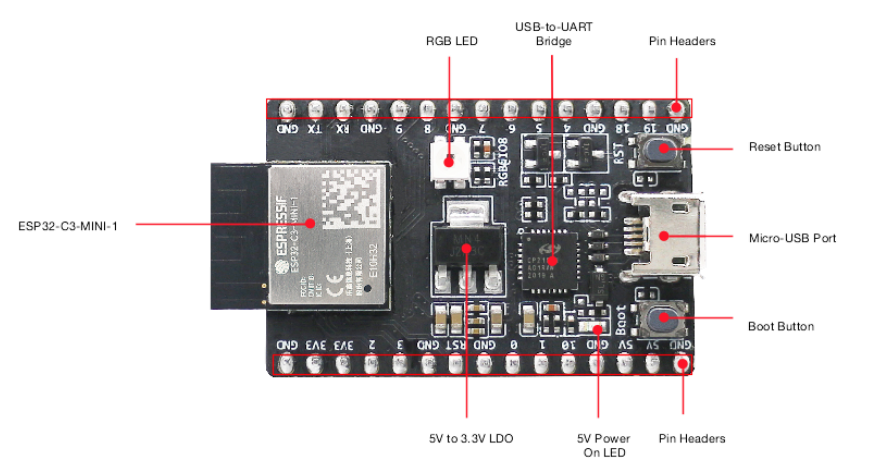
\includegraphics[scale=0.6]{imgs/esp32}
	\caption{Konfiguracija razvojnog sustava ESP32-C3-DevKitM-1 \cite{espressif}}
	\label{fig:esp32}
\end{figure}

Budući da modul ima funkciju RF (engl. \textit{radio frequency}) primopredajnika, podržava protokol Bluetooth s podrškom za velike udaljenosti. Druga važna značajka je podsustav za Wi-Fi, koji omogućava propusnost do 20 MBit/s protokolom TCP te maksimalnu propusnost od 30 MBit/s koristeći protokol UDP. 

Modul ESP32-C3-MINI-1 je bežični uređaj niske potrošnje energije (engl. ultra-low-power) primarno namijenjen razvoju aplikacija koje koriste Bluetooth Low Energy (BLE) protokol ili Wi-Fi. Na slici \ref{fig:esp32block} nalazi se blok shema modula sa svim dostupnim značajkama.

\begin{figure}[ht]
	\centering
	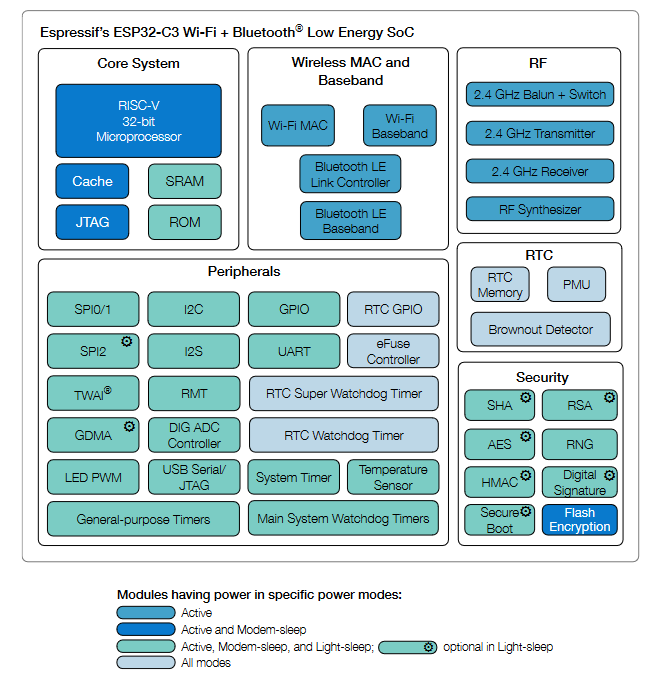
\includegraphics[scale=0.6]{imgs/esp32block}
	\caption{Blok dijagram modula ESP32-C3 \cite{esp32manual}}
	\label{fig:esp32block}
\end{figure}

\section{BLE protokol}

BLE je vrsta bežične komunikacije namijenjena komunikaciji kratkog dometa s niskom potrošnjom energije. Razvijen je kako bi se postigao standard vrlo male snage koji radi s baterijom veličine kovanice (engl. \textit{coin-cell batteries}) nekoliko godina. U odnosu na proizvode koji koriste klasičnu Bluetooth tehnologiju, BLE uređaji troše samo dio energije te omogućavaju malenim uređajima s malim baterijama bežično povezivanje s uređajima koji koriste klasični Bluetooth. \cite{blevsbluetooth}

BLE radi u istom opsegu od 2,4 GHz kao i standardni Bluetooth, no koristi različite kanale od standardnog Bluetootha. Koristi 40 kanala od 2 MHz za prijenos podataka korištenjem modulacije Gaussova pomaka frekvencije (metoda koja se koristi za glatkije prijelaze između podatkovnih impulsa), zbog čega skokovi frekvencije proizvode manje smetnji u usporedbi sa standardnom Bluetooth komunikacijom.

Atributi su adresirani dijelovi informacija koji mogu sadržavati korisničke podatke ili meta-informacije o arhitekturi samih atributa, te se koriste za razmjenu informacija između dva uređaja putem BLE sučelja. Uređaj koji prikazuje atribute naziva se poslužiteljem, a uređaj koji ih koristi naziva se klijentom. 

\eject